\documentclass[preprint,12pt]{elsarticle}
\usepackage{geometry}
%\geometry{letterpaper}                   % ... or a4paper or a5paper or ...
\usepackage{graphicx}
\usepackage{xspace}
\usepackage{amssymb} 
\usepackage{epstopdf}

 
\usepackage{datatool}
\usepackage{tikz}
\usepackage{pgfplots}
\usepackage{pgfplotstable}
\usetikzlibrary{patterns}
\usepackage{lscape}
\usepackage{subfig}
\usepackage{multirow}
\usepackage{rotating}


%% Use the option review to obtain double line spacing
%% \documentclass[preprint,review,12pt]{elsarticle}
   
%% Use the options 1p,twocolumn; 3p; 3p,twocolumn; 5p; or 5p,twocolumn
%% for a journal layout: 
%% \documentclass[final,1p,times]{elsarticle}
%% \documentclass[final,1p,times,twocolumn]{elsarticle}
%% \documentclass[final,3p,times]{elsarticle}
%% \documentclass[final,3p,times,twocolumn]{elsarticle}
%% \documentclass[final,5p,times]{elsarticle}
%% \documentclass[final,5p,times,twocolumn]{elsarticle}

%% if you use PostScript figures in your article
%% use the graphics package for simple commands
%% \usepackage{graphics}
%% or use the graphicx package for more complicated commands
%% \usepackage{graphicx}
%% or use the epsfig package if you prefer to use the old commands
%% \usepackage{epsfig}

%% The amssymb package provides various useful mathematical symbols
\usepackage{amssymb}
%% The amsthm package provides extended theorem environments
%% \usepackage{amsthm}

%% The lineno packages adds line numbers. Start line numbering with
%% \begin{linenumbers}, end it with \end{linenumbers}. Or switch it on
%% for the whole article with \linenumbers after \end{frontmatter}.
%% \usepackage{lineno}

%% natbib.sty is loaded by default. However, natbib options can be
%% provided with \biboptions{...} command. Following options are
%% valid:

%%   round  -  round parentheses are used (default)
%%   square -  square brackets are used   [option]
%%   curly  -  curly braces are used      {option}
%%   angle  -  angle brackets are used    <option>
%%   semicolon  -  multiple citations separated by semi-colon
%%   colon  - same as semicolon, an earlier confusion
%%   comma  -  separated by comma
%%   numbers-  selects numerical citations
%%   super  -  numerical citations as superscripts
%%   sort   -  sorts multiple citations according to order in ref. list
%%   sort&compress   -  like sort, but also compresses numerical citations
%%   compress - compresses without sorting
%%
%% \biboptions{comma,round}

% \biboptions{}


\journal{Journal of Systems and Software}

%%% OUR MACROS %%%
\newcommand{\COMMENT}[1]{ }

%\usepackage[usenames,dvipsnames]{xcolor}
\usepackage{xcolor}


\usepackage{amsmath}
\usepackage[thmmarks,amsmath]{ntheorem}

\newcommand{\openbox}{\leavevmode
  \hbox to.77778em{%
  \hfil\vrule
  \vbox to.675em{\hrule width.6em\vfil\hrule}%
  \vrule\hfil}}

\theoremstyle{plain}
\theoremheaderfont{\normalfont\bfseries}
\theorembodyfont{\normalfont}
\theoremseparator{}
\theoremindent0cm
\theoremnumbering{arabic}
\newtheorem{algo}{Algorithm}

\theoremstyle{plain}
%\theoremheaderfont{\normalfont\itshape}
\theoremheaderfont{\normalfont\bfseries}
\theorembodyfont{\normalfont}
\theoremseparator{}
\theoremindent0cm
\theoremnumbering{arabic}
\theoremsymbol{\ensuremath{\openbox}} 
\newtheorem{example}{Example}


\theoremstyle{plain}
\theoremheaderfont{\normalfont\bfseries}
\theorembodyfont{\normalfont}
\theoremseparator{.}
\theoremindent0cm
\theoremnumbering{arabic}
\theoremsymbol{\ensuremath{\Box}} 
\newtheorem{defi}{Definition}

\theoremstyle{plain} 
\theoremsymbol{\ensuremath{\Box}} 
\theoremseparator{.} 
\newtheorem{prop}{Property}

\def\FlyingPig{\textsl{FlyingPig}}

\newcounter{numberInTrivlist}

\newenvironment{numtrivlist}{\begin{list}{\rm \arabic{numberInTrivlist})} 
                                         {\usecounter{numberInTrivlist}
                                          \setlength{\leftmargin}{0pt}
                                          \setlength{\rightmargin}{0pt}
                                          \setlength{\itemindent}{12pt}
                                          \setlength{\listparindent}{0pt}}}
                            {\end{list}}

\newenvironment{itemizedTrivlist}{\begin{list}{\rm ~\hspace{2mm} $\bullet$\ } 
                                         {\setlength{\leftmargin}{0pt}
                                          \setlength{\rightmargin}{0pt}
                                          \setlength{\itemindent}{12pt}
                                          \setlength{\listparindent}{0pt}}}
                            {\end{list}}

\usepackage{listings}


\lstset{numbers=right, numbersep=5pt, numberstyle=\tiny, stepnumber=1,escapechar=\!,columns=fullflexible,
        morekeywords={procedure,let,for,do,if,then,else,add,choose,end,while,
        true,false,rise,exception,extend,resume,to,return,function}}

\newcommand{\pisodm}[0]{$\pi$SOD-M\xspace}

\begin{document}

\begin{frontmatter}

%% Title, authors and addresses

%% use the tnoteref command within \title for footnotes;
%% use the tnotetext command for the associated footnote;
%% use the fnref command within \author or \address for footnotes;
%% use the fntext command for the associated footnote;
%% use the corref command within \author for corresponding author footnotes;
%% use the cortext command for the associated footnote;
%% use the ead command for the email address,
%% and the form \ead[url] for the home page:
%%
%% \title{Title\tnoteref{label1}}
%% \tnotetext[label1]{}
%% \author{Name\corref{cor1}\fnref{label2}}
%% \ead{email address}
%% \ead[url]{home page}
%% \fntext[label2]{}
%% \cortext[cor1]{}
%% \address{Address\fnref{label3}}
%% \fntext[label3]{}

\title{Analyzing bibliographic collections by semi-automatizing  the systematic mapping methodology: giving quality to quantity}

%% use optional labels to link authors explicitly to addresses:
%% \author[label1,label2]{<author name>}
%% \address[label1]{<address>}
%% \address[label2]{<address>}




\author[inst1]{Pl\'acido A. Souza Neto}
\author[inst2]{Genoveva Vargas-Solar}
\author[inst3]{Umberto Souza da Costa}
\author[inst3]{Martin A. Musicante}
\author[inst2]{Javier Alfonso Espinosa-Oviedo}
\author[inst4]{Jos\'e Luis Zechinelli-Martini}
\author[inst5]{Regina Motz}
\author[inst5]{Alberto Pardo}
\author[inst5]{Agust\'in Mullin}
 
\address[inst1]{Instituto Federal do Rio Grande do Norte -- Natal, Brazil}
\address[inst2]{CNRS, LIG-LAFMIA, Saint Martin d'H\`eres, France}
\address[inst3]{Universidade Federal do Rio Grande do Norte -- Natal, Brazil}
\address[inst4]{Universidad de las Am\'ericas-Puebla, LAFMIA -- Cholula, Mexico}
\address[inst5]{Universidad de la Re\'ublica,  Montevideo, Uruguay}

\begin{abstract}

This paper discusses the results of a systematic
mapping  (SM) \cite{Petersen:2008}...

\end{abstract}

\begin{keyword}
%% keywords here, in the form: keyword \sep keyword
Data analytics \sep Semantic Web \sep Information retrieval
Provenance \sep Systematic Mapping.

%% MSC codes here, in the form: \MSC code \sep code
%% or \MSC[2008] code \sep code (2000 is the default)

\end{keyword}

\end{frontmatter}

%%
%% Start line numbering here if you want
%%
% \linenumbers

%% main text
%*********************************************************************************************************
\section{Introduction}
\label{sec:intro}
sThis paper presents a Systematic Mapping (SM)  \cite{Petersen:2008} 
about the deign of service-oriented applications in the presence of
non-functional requirements. SM is a  method for analyzing a field of interest (e.g., service oriented applications and NFR). The analysis can focus on
periodicity of publications organized by categories called facets combined to
answer  specific research questions  \cite{Budgen:2008}  that a scientist wishes to answer with quantitative data generated through the SM steps. 

The remainder of this paper is organized as follows. Section \ref{sec:background} gives
the background about NFR and service oriented applications. Section \ref{sec:mappingprocess}  describes the systematic mapping
process and our research protocol, including the search strategy and selection of papers. Section \ref{sec:outcomes} presents and interpretes the analytics results.
Section \ref{sec:conclusions} concludes the paper and discusses research perspectives. 



%..--..--..--..--..--..--..--..--..--..--..--..--..--..--..--..--..--..--..--..--..--..--..--..--..--..--..--..--..--..--..--..--..--..--..--..--..--..--
\section{Mapping process}\label{sec:mappingprocess}
%For performing our systematic mapping we adopt the method proposed in \cite{SM} consisting  of five  steps: 
\begin{enumerate}
\item \textbf{Definition of research questions}, to determine the research
scope; 
\item \textbf{Search of primary papers}, to select candidate papers expressing a   query for retrieving references from scientific
databases; 
\item \textbf{Screening of papers}, to identify relevant papers using
inclusion and exclusion criteria   to narrow
the number of papers of interest; 
\item \textbf{Keywording of abstracts}, to identify terms that are used
for producing  classification schemes named mapping categories; 
%In this step abstracts are traversed
%in the search of keywords and concepts related to the contributions
%of papers. 
%Keywords and concepts of several papers are combined to
%produce a classification scheme, namely the mapping categories. The
%classification scheme is used to unveil the structure of the research
%area. Introduction and conclusions sections have been investigated
%in the case of some papers; 
\item \textbf{Data extraction and mapping process}, to produce the systematic
mapping by clustering the papers into the mapping categories.
%Our categorization is based on publication frequencies and gives a
%broad overview of the research area. 
\end{enumerate}

%Some additional classification schemes emerged while articles were classified with respect to initial schemes because some categories were merged or splitted.

%During the sorting of articles into the classification schemes (the
%latter step), some additional classification schemes arose, some of
%them resulting from the process of merging or splitting previous mapping
%categories. 
The results of our systematic mapping are presented as
bubble plots in the next section. 
%These visual representations have two main benefits:
%first, it can easily show how the relevance of the mapping categories
%has changed over time; second, it can reveal research opportunities
%hidden on the blanks found among classification categories, pointing
%topic areas and types of publications yet to be investigated. 

%Notice that systematic mappings are complementary to systematic reviews.
%Our systematic mapping presents a broader coverage of the research
%area of interest, producing a thematic summary and disclosing the
%main scientific sources in a direct and straightforward manner. A
%systematic review can be later performed to dig into the details of
%more specific themes. 

%.........................................................
\subsection{Research questions}
\label{sec:ResearchQuestions}
%.........................................................

The  goal of our systematic mapping is to pinpoint evolutions
on the terminology of service based applications with NFR, discovering trends and the main results
produced by the community. In order to achieve this goal we formulated three research questions:
\begin{itemize}
\item {\em RQ1: Which stages of  the service-based software development process have addressed NFR?} This question is devoted to measure the evolution of publication on NFR in service-based software development and to see  which phases address NFR the most. 
\item {\em RQ2: What type of solutions have been proposed over the years to deal with NFR for service-based software?} 
This question will help us to identify how NFR are integrated within methodologies, methods, and also environments used for specifying and implementing NFR for service based applications. This question will help us to cover the publications that address particular NFR for web service based applications. It will let us identify the properties recognized by researchers as NFR according to their discipline.

\item  {\em RQ3: Which is the scope of existing solutions for addressing NFR?} NFR is a vast domain addressing different aspects according to the level of abstraction. For example, they can refer to the characteristics of the services involved in a composition (availability, reliability, economic cost), it can refer to authentication for calling services, and also to atomicity associated to the whole service composition. 


\end{itemize}


%.........................................................
\subsection{Search and Screening of Papers}

%\subsection{Expressing the  query for generating a data collection}
%.........................................................
Considering the research questions, we defined a set of keywords to be used for searching relevant works. As stated in the background, NFR are properties that represent the business rules of an application. In the early phases of the development of a Web service based application, they are stated in natural language and then they become constraints of different types in the other phases. Throughout these phases they are referred to as non-functional requirement, concern, attribute, aspect. Based on these keywords and their correlated words the query used was:

{\em ("non-functional" OR "non functional" OR quality OR NF OR QoS) AND (property OR requirement OR aspect OR attribute OR parameter OR concern OR constraint OR approach OR policy OR contract) AND ("web service" OR "service composition" OR "service based application" OR "service-based application")
}

\begin{table}\centering
\begin{tabular}{|l|c|c|c|} \hline
\textbf{Source/Action}	& \textbf{Included}	& \textbf{Excluded}	& \textbf{Total}	\\ \hline
\textit{ACM-DL}				& 33								& 56								& 89						\\ \hline
\textit{IEEE}						& 71								& 70								& 141					\\ \hline
\textit{Science Direct}	& 56								& 117							& 173					\\ \hline
\textit{CiteSeerX}			& 10								& 20								& 30						\\ \hline
\textbf{Total}					& \textbf{170}			& \textbf{263}			& \textbf{433}	\\ \hline
\end{tabular}
\caption{\label{table:Sources}Sources and number of papers.}
\end{table}

We searched and filtered relevant works in four steps. In the first  step we searched in four databases: \textit{Science Direct}\footnote{\tt http://\dots}, \textit{IEEE}\footnote{\tt http://\dots}, \textit{ACM Digital Library}\footnote{\tt http://\dots} and \textit{CiteSeerX}\footnote{\tt http://\dots} (see table \ref{table:Sources}). We retrieved 433 works. The search was done for relevant publications published between 1998 - 2014. We captured in several spreadsheets (one per database) the title, year,  and abstract of each of the references we found. During the second step we did data cleaning by excluding repeated works.  We performed another filtering procedure by reading the title and the abstract of the papers. We excluded 263 works. The columns \textbf{Included} and \textbf{Excluded} in Table~\ref{table:Sources} show the number of papers that were considered (resp. excluded) on our study.
Finally, in the last step we built   the final data collection using exclusion and inclusion criteria shown in table \ref{table:criteria}. The final data collection contained 170 papers.


\begin{table}\centering
\begin{tabular}{|l|} \hline
\textbf{Inclusion criteria}		\\ \hline\hline
- Text in English								\\ \hline
- Peer reviewed journals, conferences or workshops	\\ \hline
- PhD and master thesis	\\ \hline
- Focus on NFR for service compositions				\\ \hline\hline
\textbf{Exclusion criteria}		\\ \hline\hline	
- Abstracts, tutorials, short papers, PhD workshops, demonstrations, technical reports		\\ \hline	
- Papers dealing with service service lookup		\\ \hline
- Papers dealing with service matching 	\\ \hline
\end{tabular}
\caption{\label{table:criteria} Inclusion and exclusion criteria.}
\end{table}

%.........................................................
%\subsection{Defining classification schemes and mapping categories}
\subsection{Keywording of Abstracts} 
%.........................................................
%\textsc{Define each facet here. (including the meaning of each value).}

According to our research questions and to our interests, the papers were classified according to five analysis facets. Analysis facets are classification schemes  that define mapping categories to cluster and analyze the papers. 
The abstracts of the 170 papers included in our mapping were analyzed to discover their contribution to each of the facets defined for our study.
The result of this process is a classification of papers for the dimensions of each facet.
The results are summarized in Tables~\ref{table:biblioSPP} to~\ref{table:biblioMTMM}.
The six facets with the associated classified references of our SM are described as in the following lines. 
%\begin{itemize}
%\paragraph {\bf\em Research type}, refers to the contribution type reported by a reference: {\em validation} , {\em evaluation} ,	{\em solution},	{philosophical} discussion, {\em	opinion} (position paper)	and {\em experience} report.

%_____________________________________________________
\paragraph {\bf\em Software process phase} 
%_____________________________________________________
refers to papers that address the specification of NFR during a given software process phase: {\em specification},	 {\em design},	{\em implementation},	{\em tests},	{\em validation}	and {\em maintenance}.

\begin{table}\centering
\footnotesize
\begin{tabular}{|c|c|}\hline
\textbf{Dimension} & \textbf{References} \\ \hline
%\multirow{6}{*}{\begin{sideways} \textbf{Sw Pr Phase} \end{sideways} } & 
%\\ \cline{2-3}
Specification	& 
\parbox{0.6\textwidth}{\cite{p005}, \cite{p006}, \cite{p009}, \cite{p012}, \cite{p013}, \cite{p016},  \cite{p017}, \cite{p018}, \cite{p019}, \cite{p020}, \cite{p021}, \cite{p023}, \cite{p024}, \cite{p026},  \cite{p034}, \cite{p036}, \cite{p037}, \cite{p041}, \cite{p043}, \cite{p044}, \cite{p045}, \cite{p046},  \cite{p047}, \cite{p048}, \cite{p055}, \cite{p069}, \cite{p076}, \cite{p077}, \cite{p078}, \cite{p090},  \cite{p091}, \cite{p092}, \cite{p098}, \cite{p099}, \cite{p100}, \cite{p105}, \cite{p109}, \cite{p112},  \cite{p116}, \cite{p118}, \cite{p119}, \cite{p123}, \cite{p124}, \cite{p129}, \cite{p130}, \cite{p131},  \cite{p132}, \cite{p133}, \cite{p134}, \cite{p135}, \cite{p136}, \cite{p146}, \cite{p149}, \cite{p151}.}
\\ \hline
Design		&
\parbox{0.6\textwidth}{\cite{p001}, \cite{p002}, \cite{p003}, \cite{p004}, \cite{p005}, \cite{p007},  \cite{p008}, \cite{p009}, \cite{p010}, \cite{p011}, \cite{p012}, \cite{p014}, \cite{p015}, \cite{p016},  \cite{p017}, \cite{p018}, \cite{p020}, \cite{p023}, \cite{p024}, \cite{p025}, \cite{p026}, \cite{p027},  \cite{p029}, \cite{p031}, \cite{p032}, \cite{p034}, \cite{p036}, \cite{p037}, \cite{p044}, \cite{p046},  \cite{p049}, \cite{p052}, \cite{p053}, \cite{p054}, \cite{p056}, \cite{p057}, \cite{p059}, \cite{p064}, \cite{p065}, \cite{p066}, \cite{p067}, \cite{p069}, \cite{p070}, \cite{p073}, \cite{p074}, \cite{p078}, \cite{p079}, \cite{p080}, \cite{p083}, \cite{p084}, \cite{p085}, \cite{p086}, \cite{p089}, \cite{p091},  \cite{p093}, \cite{p094}, \cite{p095}, \cite{p096}, \cite{p097}, \cite{p098}, \cite{p099}, \cite{p100}, \cite{p101}, \cite{p102}, \cite{p103}, \cite{p104}, \cite{p105}, \cite{p109}, \cite{p110}, \cite{p118}, \cite{p119}, \cite{p120}, \cite{p121}, \cite{p122}, \cite{p124}, \cite{p125}, \cite{p126}, \cite{p127}, \cite{p128}, \cite{p129}, \cite{p130}, \cite{p136}, \cite{p138}, \cite{p139}, \cite{p145}, \cite{p147}, \cite{p148}, \cite{p149}, \cite{p150}, \cite{p151}, \cite{p152}, \cite{p153}, \cite{p154}, \cite{p155}, \cite{p156}, \cite{p157}, \cite{p162}, \cite{p163}, \cite{p165}, \cite{p166}, \cite{p168}, \cite{p169}, \cite{p170}.}
\\ \hline
Implementation		&
\parbox{0.6\textwidth}{\cite{p001}, \cite{p008}, \cite{p020}, \cite{p021}, \cite{p022}, \cite{p029}, \cite{p030}, \cite{p032}, \cite{p033}, \cite{p039}, \cite{p040}, \cite{p046}, \cite{p049}, \cite{p050}, \cite{p051}, \cite{p053}, \cite{p054}, \cite{p058}, \cite{p059}, \cite{p060}, \cite{p062}, \cite{p063}, \cite{p064}, \cite{p065}, \cite{p068}, \cite{p071}, \cite{p072}, \cite{p073}, \cite{p075}, \cite{p079}, \cite{p080}, \cite{p081}, \cite{p086}, \cite{p087}, \cite{p096}, \cite{p105}, \cite{p106}, \cite{p107}, \cite{p111}, \cite{p113}, \cite{p114}, \cite{p115}, \cite{p116}, \cite{p117}, \cite{p119}, \cite{p121}, \cite{p122}, \cite{p124}, \cite{p125}, \cite{p126}, \cite{p137}, \cite{p138}, \cite{p142}, \cite{p143}, \cite{p144}, \cite{p145}, \cite{p151}, \cite{p158}, \cite{p159}, \cite{p160}, \cite{p161}, \cite{p167},\cite{p169}.}
\\ \hline
Tests	&	
\parbox{0.6\textwidth}{\cite{p105}, \cite{p108}, \cite{p124}.}
\\ \hline
Validation	&	
\parbox{0.6\textwidth}{\cite{p021}, \cite{p035}, \cite{p076}, \cite{p105}, \cite{p112}, \cite{p114}\cite{p124}, \cite{p140}.}
\\ \hline
Manteinance &	
\parbox{0.6\textwidth}{\cite{p028}, \cite{p030}, \cite{p033}, \cite{p038}, \cite{p080}, \cite{p081}, \cite{p082}, \cite{p086}, \cite{p087}, \cite{p089}, \cite{p107}, \cite{p109}, \cite{p113}, \cite{p122}, \cite{p124}, \cite{p141}, \cite{p160}.}
\\ \hline
\end{tabular}
\caption{\label{table:biblioSPP} Facet: Software Process Phase.}
\end{table}

%_____________________________________________________
\paragraph {\bf\em Contribution} 
%_____________________________________________________
refers to the concrete result described in a reference: {\em language},	{\em method}, 	{\em tool}, {\em 	composition algorithm}, {\em	model}, and	{\em process}.
\begin{table}\centering
\footnotesize
\begin{tabular}{|c|c|}\hline
\textbf{Dimension} & \textbf{References} \\ \hline
%\multirow{6}{*}{\begin{sideways} \textbf{Sw Pr Phase} \end{sideways} } & 
%\\ \cline{2-3}
Language	& 
\parbox{0.6\textwidth}{\cite{p006}, \cite{p019}, \cite{p033}, \cite{p046}, \cite{p050}, \cite{p058}, \cite{p067}, \cite{p069}, \cite{p083}, \cite{p087}, \cite{p090},  \cite{p098}, \cite{p099}, \cite{p100}, \cite{p109}, \cite{p149}, \cite{p151}.}
\\ \hline
Method	& 
\parbox{0.6\textwidth}{\cite{p008}, \cite{p010}, \cite{p012}, \cite{p015}, \cite{p016},  \cite{p017}, \cite{p023}, \cite{p025}, \cite{p035}, \cite{p036}, \cite{p037}, \cite{p043}, \cite{p044}, \cite{p045}, \cite{p048}, \cite{p065}, \cite{p077}, \cite{p078}, \cite{p079}, \cite{p082}, \cite{p084}, \cite{p085},  \cite{p086}, \cite{p089}, \cite{p093}, \cite{p095}, \cite{p102}, \cite{p108}, \cite{p112}, \cite{p115}, \cite{p118}, \cite{p119}, \cite{p134}, \cite{p135}, \cite{p138}, \cite{p140}, \cite{p143}, \cite{p146}, \cite{p147}, \cite{p148}, \cite{p149}, \cite{p151}, \cite{p154}, \cite{p166}.}
\\ \hline
Tool		&
\parbox{0.6\textwidth}{\cite{p007},  \cite{p009}, \cite{p020}, \cite{p021}, \cite{p030}, \cite{p032}, \cite{p038}, \cite{p039}, \cite{p057}, \cite{p059}, \cite{p063}, \cite{p064}, \cite{p066}, \cite{p071}, \cite{p073}, \cite{p075}, \cite{p076}, \cite{p080}, \cite{p081}, \cite{p091}, \cite{p094}, \cite{p105}, \cite{p106}, \cite{p107}, \cite{p111}, \cite{p113}, \cite{p114}, \cite{p116}, \cite{p121}, \cite{p122}, \cite{p124}, \cite{p125}, \cite{p126}, \cite{p129}, \cite{p130}, \cite{p151}, \cite{p156}, \cite{p158}, \cite{p159}, \cite{p160}, \cite{p165}, \cite{p167}, \cite{p169}.}
\\ \hline
Composition Algorithm		&
\parbox{0.6\textwidth}{\cite{p001}, \cite{p002}, \cite{p003}, \cite{p004}, \cite{p007}, \cite{p008}, \cite{p018}, \cite{p026}, \cite{p027}, \cite{p051}, \cite{p060}, \cite{p062}, \cite{p068}, \cite{p092}, \cite{p097}, \cite{p103}, \cite{p104}, \cite{p116}, \cite{p117}, \cite{p118}, \cite{p120}, \cite{p122}, \cite{p123}, \cite{p125}, \cite{p127}, \cite{p131}, \cite{p132}, \cite{p133}, \cite{p137}, \cite{p144}, \cite{p145}, \cite{p153}, \cite{p155}, \cite{p157}, \cite{p165}.}
\\ \hline
Model	&	
\parbox{0.6\textwidth}{\cite{p005}, \cite{p013}, \cite{p018}, \cite{p022}, \cite{p024}, \cite{p034}, \cite{p055}, \cite{p056}, \cite{p070}, \cite{p072}, \cite{p110}, \cite{p114}, \cite{p150}, \cite{p163}, \cite{p168}.}
\\ \hline
Process	&	
\parbox{0.6\textwidth}{\cite{p009}, \cite{p011}, \cite{p014}, \cite{p023}, \cite{p028}, \cite{p029}, \cite{p031}, \cite{p040}, \cite{p047}, \cite{p049}, \cite{p053}, \cite{p061}, \cite{p074}, \cite{p096}, \cite{p124}, \cite{p128}, \cite{p136}, \cite{p139}, \cite{p141}, \cite{p142}, \cite{p152}, \cite{p161}, \cite{p162}, \cite{p170}.}
\\ \hline
\end{tabular}
\caption{\label{table:biblioContrib} Facet: Contribution.}
\end{table}

%_____________________________________________________
\paragraph {\bf\em Paradigm} 
%_____________________________________________________
refers to the modelling paradigm used to design NFR for service based applications: {\em model-driven},	{\em middleware}, {\em aspect oriented},	{\em service process language},		{\em semantic}, 	{\em traditional}, {\em other}.

\begin{table}\centering
\footnotesize
\begin{tabular}{|c|c|}\hline
\textbf{Dimension} & \textbf{References} \\ \hline
%\multirow{6}{*}{\begin{sideways} \textbf{Sw Pr Phase} \end{sideways} } & 
%\\ \cline{2-3}
Model-Driven	& 
\parbox{0.6\textwidth}{\cite{p006}, \cite{p039}, \cite{p064}, \cite{p065}, \cite{p085}, \cite{p086}, \cite{p087}, \cite{p096}, \cite{p110}, \cite{p119}, \cite{p125}, \cite{p149}.
}
\\ \hline
Middleware	& 
\parbox{0.6\textwidth}{\cite{p002}, \cite{p005}, \cite{p011}, \cite{p013}, \cite{p014}, \cite{p016},  \cite{p018}, \cite{p019}, \cite{p020}, \cite{p022}, \cite{p029}, \cite{p030}, \cite{p032}, \cite{p033}, \cite{p038}, \cite{p053}, \cite{p062}, \cite{p076}, \cite{p082}, \cite{p095}, \cite{p096}, \cite{p105}, \cite{p111}, \cite{p113}, \cite{p114}, \cite{p116},  \cite{p126}, \cite{p127}, \cite{p153}, \cite{p156}, \cite{p162}, \cite{p167}, \cite{p169}.
}
\\ \hline
Aspect-Oriented		&
\parbox{0.6\textwidth}{\cite{p022}, \cite{p038}, \cite{p039}, \cite{p042}, \cite{p046}, \cite{p080}, \cite{p086}, \cite{p099}, \cite{p100}, \cite{p120}, \cite{p151}.
}
\\ \hline
Software Product Line		&
\parbox{0.6\textwidth}{\cite{p124}, \cite{p145}.
}
\\ \hline
Semantic	&	
\parbox{0.6\textwidth}{\cite{p014}, \cite{p015}, \cite{p016},  \cite{p023}, \cite{p044}, \cite{p046}, \cite{p049}, \cite{p054}, \cite{p069}, \cite{p073}, \cite{p080}, \cite{p092}, \cite{p105}, \cite{p106}, \cite{p109}, \cite{p116},  \cite{p117}, \cite{p121}, \cite{p123}, \cite{p139}, \cite{p156}, \cite{p165}, \cite{p168}.
}
\\ \hline
Traditional	&	
\parbox{0.6\textwidth}{\cite{p026}, \cite{p027}, \cite{p037}, \cite{p048}, \cite{p052}, \cite{p083}, \cite{p098}, \cite{p127}, \cite{p129}, \cite{p138}.
}
\\ \hline
Other	&	
\parbox{0.6\textwidth}{\cite{p001}, \cite{p003}, \cite{p004}, \cite{p007}, \cite{p008}, \cite{p009}, \cite{p010}, \cite{p012}, \cite{p017}, \cite{p021}, \cite{p024}, \cite{p025}, \cite{p028}, \cite{p031}, \cite{p034}, \cite{p035}, \cite{p036}, \cite{p040}, \cite{p047}, \cite{p050}, \cite{p051}, \cite{p055}, \cite{p056}, \cite{p057}, \cite{p058}, \cite{p059}, \cite{p060}, \cite{p061}, \cite{p063}, \cite{p066}, \cite{p067}, \cite{p068}, \cite{p070}, \cite{p071}, \cite{p072}, \cite{p074}, \cite{p075}, \cite{p077}, \cite{p078}, \cite{p079}, \cite{p084}, \cite{p091}, \cite{p097}, \cite{p112}, \cite{p118}, \cite{p133}, \cite{p137}, \cite{p141}, \cite{p142}, \cite{p143}, \cite{p144}, \cite{p146}, \cite{p147}, \cite{p148}, \cite{p151}.
}
\\ \hline
\end{tabular}
\caption{\label{table:biblioPara} Facet: Paradigm.}
\end{table}

%_____________________________________________________
\paragraph {\bf\em Technique} 
%_____________________________________________________
refers to the formal or empirical tool used to develop a solution to deal with NFR within service based applications:  {\em heuristics / optimization},	{\em graphs / planning},	{\em genetic algorithm / genetic programming}	, {\em Petri nets},	{\em formal method},	{\em automata},	{\em agents},	and {\em ad-hoc / other}.

\begin{table}\centering
\footnotesize
\begin{tabular}{|c|c|}\hline
\textbf{Dimension} & \textbf{References} \\ \hline
%\multirow{6}{*}{\begin{sideways} \textbf{Sw Pr Phase} \end{sideways} } & 
%\\ \cline{2-3}
Heuristics/Optimization	& 
\parbox{0.6\textwidth}{
\cite{p001}, \cite{p003}, \cite{p004}, \cite{p007}, \cite{p008}, \cite{p011}, \cite{p015}, \cite{p016},  \cite{p025}, \cite{p026}, \cite{p033}, \cite{p036}, \cite{p037}, \cite{p048}, \cite{p056}, \cite{p060}, \cite{p077}, \cite{p079}, \cite{p081}, \cite{p082}, \cite{p084}, \cite{p085}, \cite{p095}, \cite{p102}, \cite{p103}, \cite{p104}, \cite{p106}, \cite{p118}, \cite{p122}, \cite{p123}, \cite{p125}, \cite{p127}, \cite{p128}, \cite{p129}, \cite{p130}, \cite{p131}, \cite{p132}, \cite{p133}, \cite{p135}, \cite{p139}, \cite{p145}, \cite{p148}, \cite{p154}, \cite{p155}, \cite{p158}, \cite{p161}, \cite{p166}, \cite{p167}, \cite{p170}.
}
\\ \hline
Graphs/Planning	& 
\parbox{0.6\textwidth}{
\cite{p010}, \cite{p072}, \cite{p116}, \cite{p142}, \cite{p143}, \cite{p152}, \cite{p167}.
}
\\ \hline
Evolutionary Techniques		&
\parbox{0.6\textwidth}{
\cite{p008}, \cite{p009}, \cite{p020}, \cite{p030}, \cite{p031}, \cite{p032}, \cite{p036}, \cite{p051}, \cite{p068}, \cite{p113}, \cite{p117}, \cite{p125}, \cite{p137}, \cite{p147}.
}
\\ \hline
Formal Methods	&
\parbox{0.6\textwidth}{
\cite{p027}, \cite{p041}, \cite{p055}, \cite{p070}, \cite{p090}, \cite{p092}, \cite{p097}, \cite{p104}, \cite{p112}, \cite{p136}, \cite{p165}.
}
\\ \hline
Automata/Petri Nets	&	
\parbox{0.6\textwidth}{
\cite{p013}, \cite{p028}, \cite{p091}, \cite{p104}, \cite{p140}, \cite{p160}.
}
\\ \hline
Agents	&	
\parbox{0.6\textwidth}{
\cite{p014}, \cite{p078}, \cite{p141}.
}
\\ \hline
\textit{Ad-hoc}/Other	&	
\parbox{0.6\textwidth}{
\cite{p002}, \cite{p004}, \cite{p005}, \cite{p006}, \cite{p009}, \cite{p012}, \cite{p015}, \cite{p018}, \cite{p019}, \cite{p021}, \cite{p023}, \cite{p024}, \cite{p029}, \cite{p034}, \cite{p035}, \cite{p040}, \cite{p044}, \cite{p047}, \cite{p049}, \cite{p050}, \cite{p052}, \cite{p053}, \cite{p057}, \cite{p058}, \cite{p059}, \cite{p061}, \cite{p062}, \cite{p063}, \cite{p064}, \cite{p065}, \cite{p066}, \cite{p067}, \cite{p069}, \cite{p071}, \cite{p073}, \cite{p074}, \cite{p075}, \cite{p076}, \cite{p080}, \cite{p083}, \cite{p094}, \cite{p096}, \cite{p098}, \cite{p100}, \cite{p119}, \cite{p122}, \cite{p128}, \cite{p134}, \cite{p138}, \cite{p146}, \cite{p147}, \cite{p149}, \cite{p150}, \cite{p151}, \cite{p153}, \cite{p156}, \cite{p157}, \cite{p159}, \cite{p163}, \cite{p168}.
}
\\ \hline
\end{tabular}
\caption{\label{table:biblioMTMM} Facet: Main Technique/Mathematical Model.}
\end{table}

%_____________________________________________________
\paragraph{\bf\em NFR type} 
%_____________________________________________________
refers to the types identified by the ISO/IEC 9126 ({\em functionality, reliability, usability, efficiency, maintainability, portability}) and it also includes  {\em local/global } and {\em QoS as general parameter}. Each ISO NFR type has associated dimensions that defines it.  The {\em functionality}  refers to suitability, accuracy, interoperability, security, and functionality compliance.	The {\em reliability} of a system is defined by its  maturity, fault tolerance, recoverability, reliability compliance.	The {\em usability} of a system is defined by its understandability, learnability, operability, attractiveness, and usability compliance. The	{\em efficiency} of a system is defined by its  time behaviour, resource utilization,  and efficiency compliance.	The {\em maintainability} of a system is defined by its analyzability, changeability, stability, testability and maintainability compliance.	The {\em portability} of a system is defined by its adaptability, installability, co-existence, replaceability, and portability compliance.					
%\end{itemize}

\begin{table}\centering
\footnotesize
\begin{tabular}{|c|c|}\hline
\textbf{Dimension} & \textbf{References} \\ \hline
%\multirow{6}{*}{\begin{sideways} \textbf{Sw Pr Phase} \end{sideways} } & 
%\\ \cline{2-3}
Functionality	& 
\parbox{0.6\textwidth}{
\cite{p022}, \cite{p026}, \cite{p050}, \cite{p062}, \cite{p063}, \cite{p118}, \cite{p119}, \cite{p120}, \cite{p138}, \cite{p140}, \cite{p147}, \cite{p149}, \cite{p168}.
}
\\ \hline
Reliability	& 
\parbox{0.6\textwidth}{
\cite{p012}, \cite{p017}, \cite{p026}, \cite{p062}, \cite{p063}, \cite{p116}, \cite{p118}, \cite{p122}, \cite{p133}, \cite{p147}, \cite{p149}, \cite{p150}, \cite{p152}, \cite{p166}.
}
\\ \hline
Usability	&
\parbox{0.6\textwidth}{
\cite{p027}, \cite{p138}, \cite{p147}, \cite{p149}, \cite{p152}.
}
\\ \hline
Efficiency	&
\parbox{0.6\textwidth}{
\cite{p017}, \cite{p026}, \cite{p027}, \cite{p050}, \cite{p062}, \cite{p064}, \cite{p115}, \cite{p118}, \cite{p120}, \cite{p124}, \cite{p138}, \cite{p147}, \cite{p149}, \cite{p150}, \cite{p152}, \cite{p160}, \cite{p166}, \cite{p168}.
}
\\ \hline
Maintainability	&	
\parbox{0.6\textwidth}{
\cite{p147}, \cite{p149}, \cite{p152}.
}
\\ \hline
Portability	&	
\parbox{0.6\textwidth}{
\cite{p122}, \cite{p147}, \cite{p149}, \cite{p152}.
}
\\ \hline
Local/Global QoS	&	
\parbox{0.6\textwidth}{
\cite{p013}, \cite{p015}, \cite{p044}, \cite{p048}, \cite{p056}, \cite{p076}, \cite{p081}, \cite{p091}, \cite{p092}, \cite{p093}, \cite{p095}, \cite{p110}, \cite{p114}, \cite{p129}, \cite{p130}, \cite{p132}, \cite{p134}, \cite{p135}, \cite{p139}, \cite{p141}, \cite{p142}, \cite{p161}, \cite{p163}, \cite{p166}.
}
\\ \hline
QoS treated as a general parameter	&	
\parbox{0.6\textwidth}{
\cite{p001}, \cite{p002}, \cite{p003}, \cite{p004}, \cite{p005}, \cite{p006}, \cite{p007}, \cite{p008}, \cite{p009}, \cite{p010}, \cite{p011}, \cite{p014}, \cite{p016}, \cite{p018}, \cite{p019}, \cite{p021}, \cite{p023}, \cite{p024}, \cite{p025}, \cite{p028}, \cite{p029}, \cite{p030}, \cite{p031}, \cite{p032}, \cite{p033}, \cite{p034}, \cite{p035}, \cite{p036}, \cite{p038}, \cite{p039}, \cite{p040}, \cite{p042}, \cite{p046}, \cite{p047}, \cite{p048}, \cite{p049}, \cite{p051}, \cite{p052}, \cite{p053}, \cite{p054}, \cite{p055}, \cite{p057}, \cite{p058}, \cite{p059}, \cite{p060}, \cite{p061}, \cite{p065}, \cite{p066}, \cite{p067}, \cite{p068}, \cite{p069}, \cite{p070}, \cite{p071}, \cite{p073}, \cite{p074}, \cite{p075}, \cite{p076}, \cite{p077}, \cite{p078}, \cite{p079}, \cite{p080}, \cite{p082}, \cite{p083}, \cite{p084}, \cite{p085}, \cite{p086}, \cite{p087}, \cite{p088}, \cite{p089}, \cite{p090}, \cite{p094}, \cite{p096}, \cite{p097}, \cite{p098}, \cite{p099}, \cite{p100}, \cite{p101}, \cite{p102}, \cite{p103}, \cite{p104}, \cite{p105}, \cite{p106}, \cite{p107}, \cite{p108}, \cite{p109}, \cite{p111}, \cite{p112}, \cite{p113}, \cite{p117}, \cite{p121}, \cite{p123}, \cite{p124}, \cite{p125}, \cite{p126}, \cite{p127}, \cite{p128}, \cite{p131}, \cite{p134}, \cite{p137}, \cite{p140}, \cite{p143}, \cite{p144}, \cite{p145}, \cite{p146}, \cite{p148}, \cite{p151}, \cite{p153}, \cite{p154}, \cite{p155}, \cite{p156}, \cite{p157}, \cite{p158}, \cite{p159}, \cite{p162}, \cite{p163}, \cite{p164}, \cite{p165}, \cite{p167}, \cite{p169}, \cite{p170}.
}
\\ \hline
\end{tabular}
\caption{\label{table:biblioMTMM} Facet: NFR Type-ISO/IEC 9126 (Extended).}
\end{table}


We analyzed data quantitatively by reading the papers and by clustering them according to the facets. The following section shows the analysis results and answers our research questions.
%..--..--..--..--..--..--..--..--..--..--..--..--..--..--..--..--..--..--..--..--..--..--..--..--..--..--..--..--..--..--..--..--..--..--..--..--..--..--

%..--..--..--..--..--..--..--..--..--..--..--..--..--..--..--..--..--..--..--..--..--..--..--..--..--..--..--..--..--..--..--..--..--..--..--..--..--..--
\section{Outcomes}
\label{sec:outcomes}
%
This section is devoted to the analysis and discussion of the results for our systematic mapping.
We proceed by \textit{(i)} presenting the collected data in a graphic form and \textit{(ii)} answering the research questions for our study.

%...............................................................................................................................................................
\subsection{Quantitative analysis}
%...............................................................................................................................................................
Our quantitative analysis of the results shows the  
frequencies of publications for each facet. Results have been aggregated in bullet charts (see  Figure~\ref{fig:publisherperyear}).
\begin{figure}
  \centering
  \subfloat[Publisher per Year]
  {\label{fig:publisherperyear}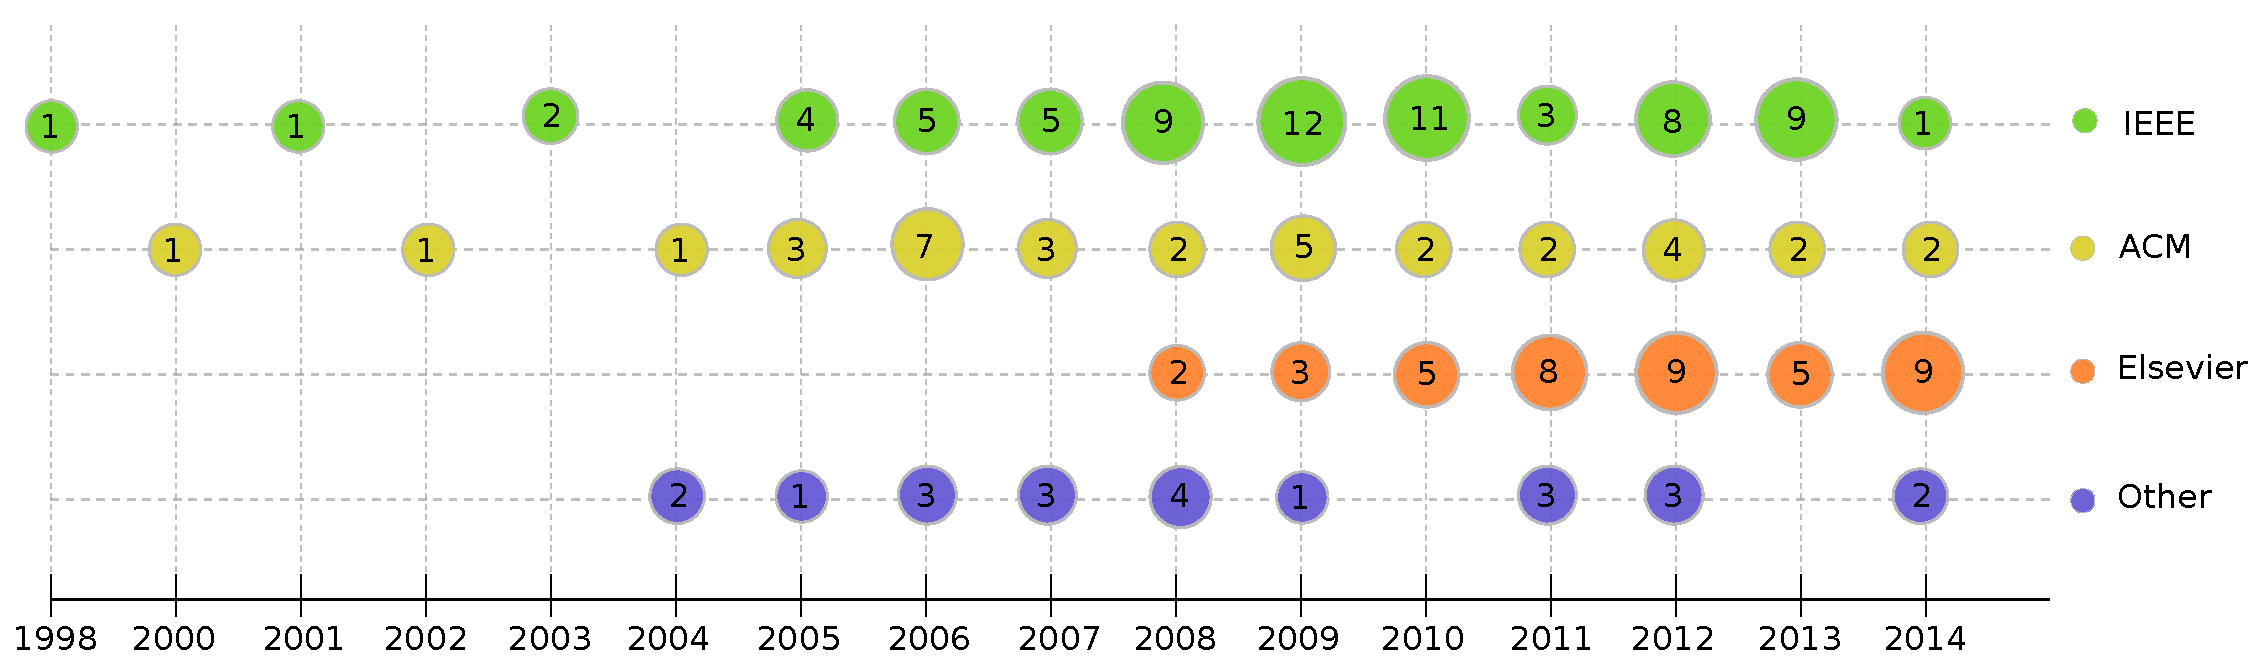
\includegraphics[width=0.99\textwidth]{figs/PublisherPerYear}}
  ~ %add desired spacing between images, e. g. ~, \quad, \qquad etc. (or a blank line to force the subfig onto a new line)
  \\
  \subfloat[Contribution per Year]
  {\label{fig:contributionperyear}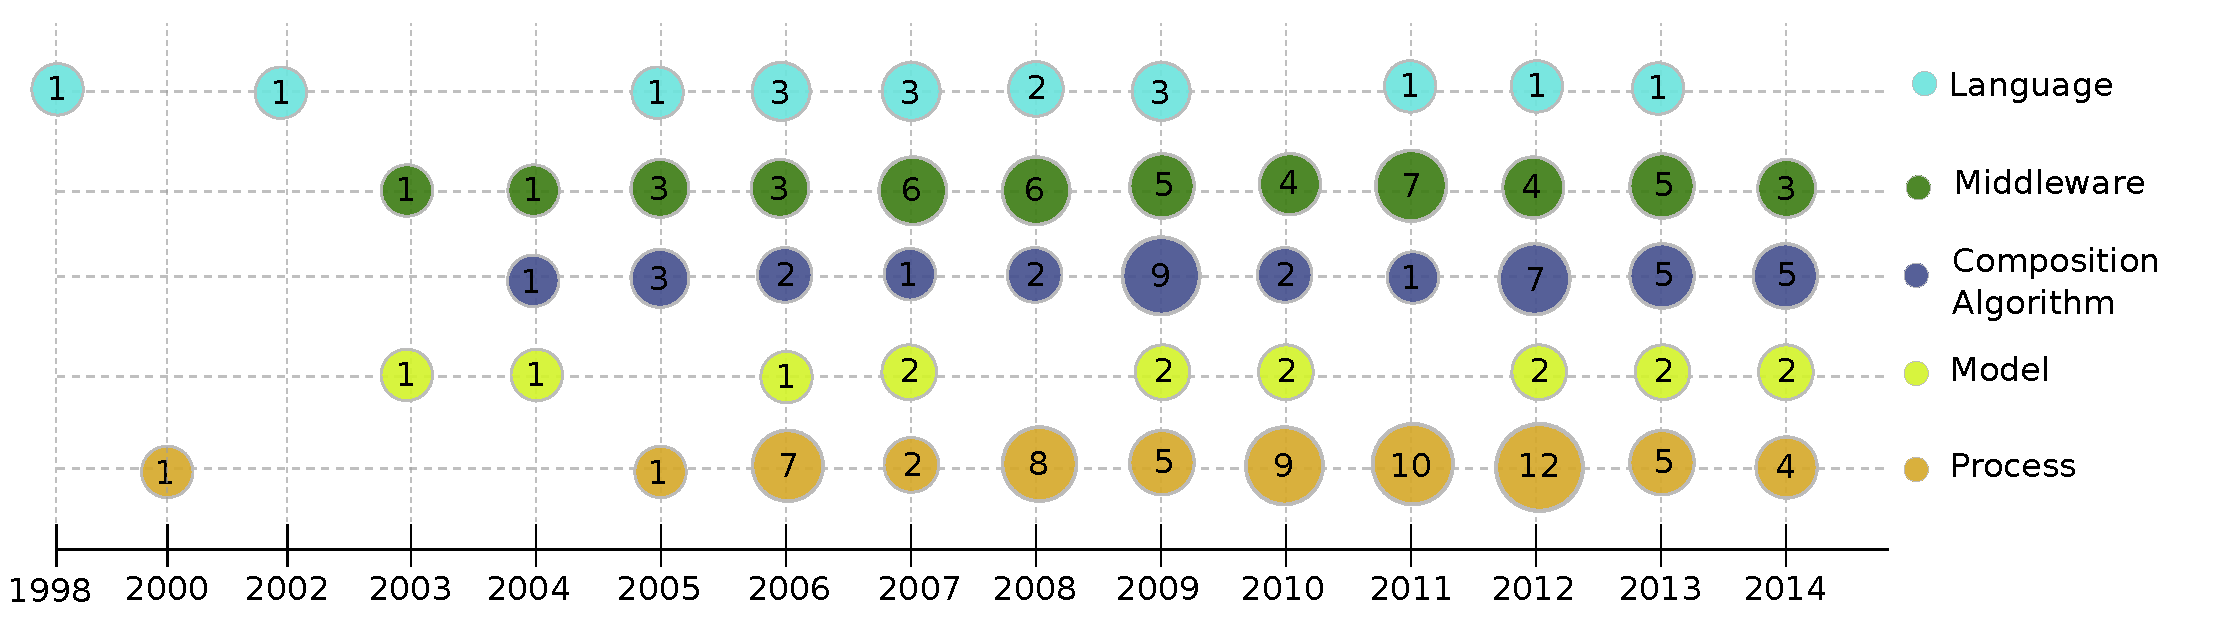
\includegraphics[width=0.99\textwidth]{figs/ContributionPerYear}}
   %add desired spacing between images, e. g. ~, \quad, \qquad etc. (or a blank line to force the subfig onto a new line)
  ~
  \\
  \subfloat[Paradigm per Year]
  {\label{fig:paradigmperyear}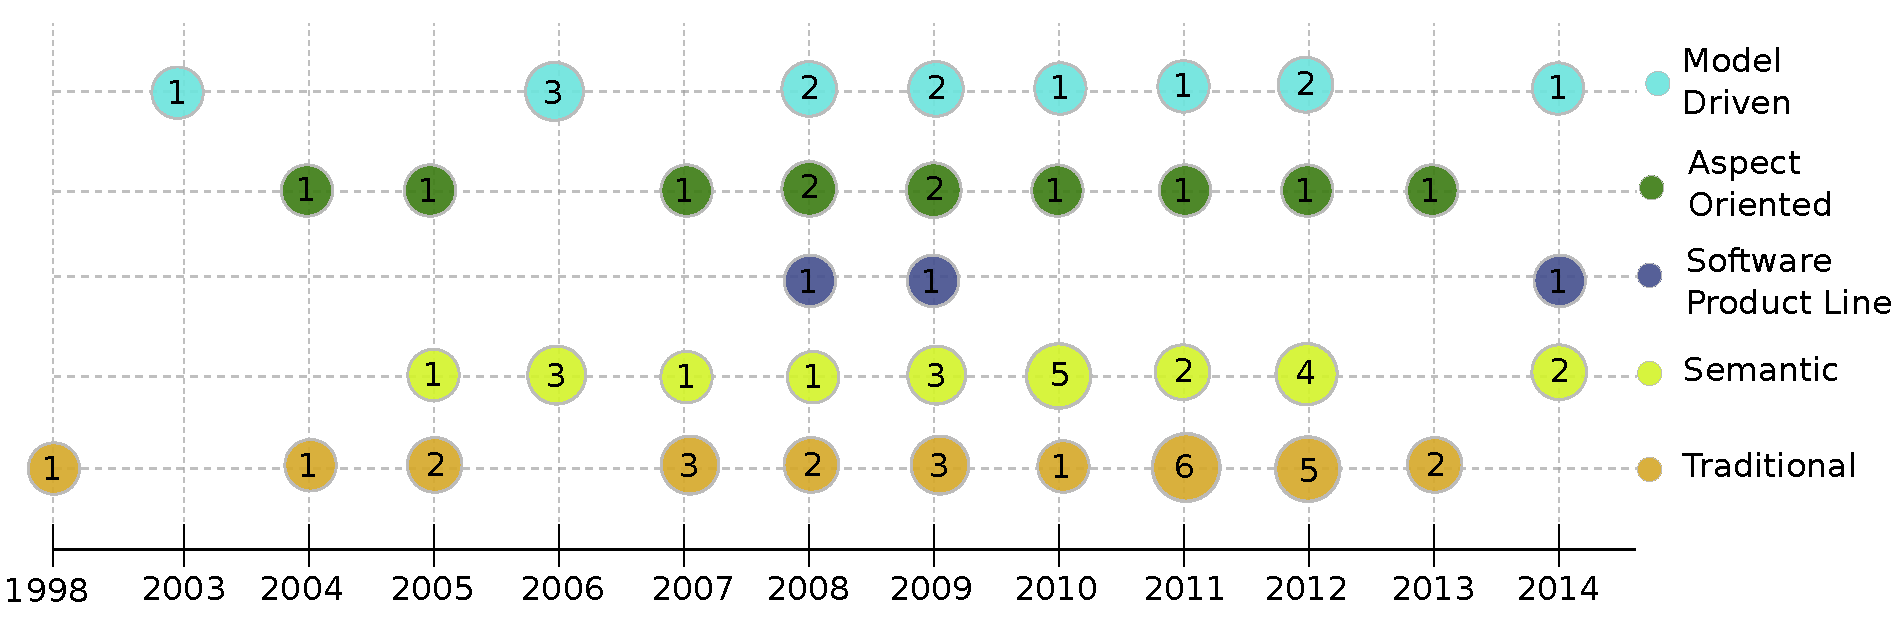
\includegraphics[width=0.99\textwidth]{figs/ParadigmPerYearNew}}
  ~ %add desired spacing between images, e. g. ~, \quad, \qquad etc. (or a blank line to force the subfig onto a new line)

  \caption{Publications per Year}
  \label{fig:publicationsperyear}
\end{figure}

We computed bubble charts that aggregate the number of papers published by year in the area (see
Figure \ref{fig:publicationsperyear}).  The following  presents the aggregated view of the number of papers published by year and by facet.

Despite  the low number of works tackling \textit{other} publishers, they
maintain their presence over the years,  mainly between 2008-2014. IEEE and ACM are
the publishers that most published papers related to service-oriented
applications considering non-functional properties. Considering Elsevier, we can
found papers only from 2008. Figure \ref{fig:publisherperyear} presents the
publications for each publisher per year.    

Figure \ref{fig:contributionperyear} presents the distribution of papers per
contribution category by year. As shown in the figure, particularly between 2008 and 2012 most papers propose a middleware and a process, while composition algorithms were mainly published in 2008 and 2012. Papers proposing \textit{SPL} are not numerous but the number remains stable along the years, while semantic and traditional proposals are quite popular.

 
 %......................................................................................
\subsection{Analysis by combining facets}
%......................................................................................
For the analysis, we computed the
volume of publications by publisher (Figure \ref{fig:publisherperyear}). We
also analyzed the publications considering the facets 
{\em contribution} and {\em paradigm} as pivot references that can be then put in perspectives by combining them with the other three facets (see Figures \ref{fig:contributionperyear} and
\ref{fig:paradigmperyear}).
The facet contribution   serves to organize papers that propose solutions for modelling, expressing and implementing NFR for service-based applications (Figures
\ref{fig:Facets-Contribution-ProcessParadigm}, 
\ref{fig:Facets-Contribution-MatematicalModel} and
\ref{fig:Facets-Contribution-NFR}). The facet paradigm serves to organize papers that propose methodologies for implementing service based software with  NFR (Figure \ref{fig:Facets-Paradigm-ContributionProcess}). 

%......................................................................................
\subsubsection{Contribution - Process - Paradigm facets}
%......................................................................................
\begin{figure} [htpb]
\centering
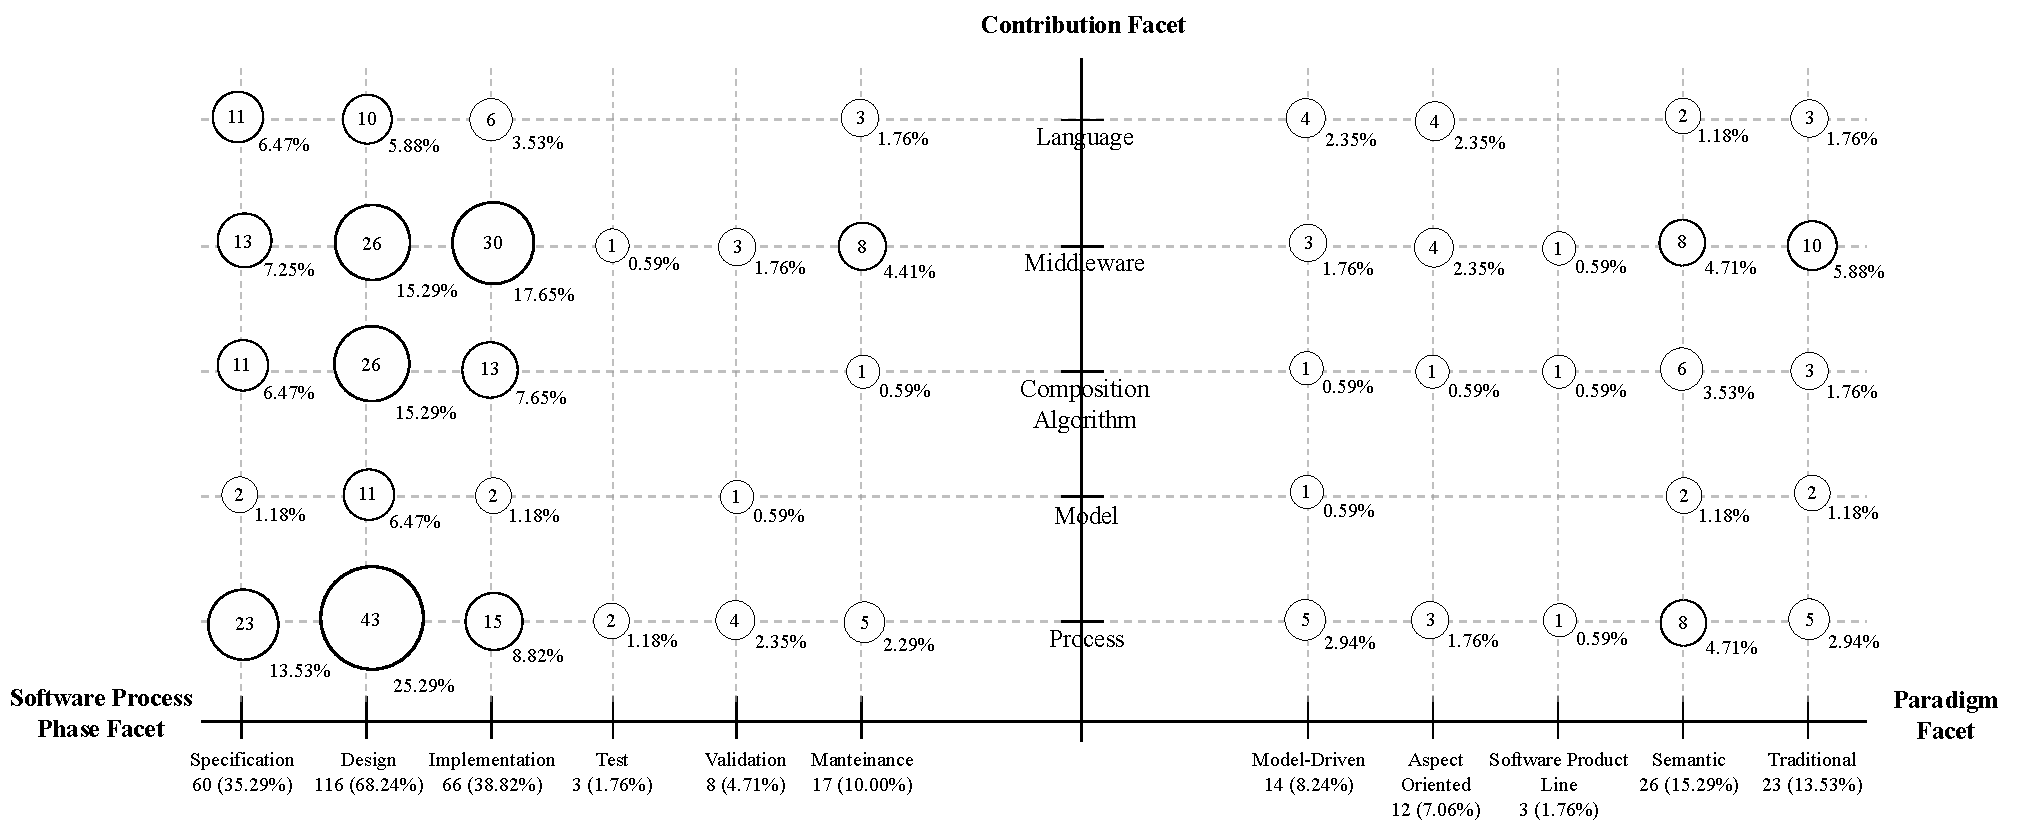
\includegraphics[width=0.99\textwidth]{figs/Facets-Contribution-ProcessParadigm}
\caption{Facet Contribution with facets Software development process and Paradigm }
\label{fig:Facets-Contribution-ProcessParadigm}
\end{figure}   

We combined the facet {\em contribution} with the facets {\em process} and {\em paradigm} to try to observe the relationship between the contribution associated to software development phase and the type of contribution reported in a paper (see
Figure
\ref{fig:Facets-Contribution-ProcessParadigm}). We observed that NFR are rarely considered in the test, validation and maintenance phases of a service-based software development methodology. There are 8 papers that relate
middleware (contribution) with the maintenance phase in their  proposals. 
Specification (35.29\%), Design (68.24\%) and Implementation
(38.82\%)\footnote{There are papers which were classified in more than one
category, considering all facets, \textit{e.g.}, one paper may be classified
in design and implementation; or middleware and composition algorithm.} are the phases most frequently addressed in papers.
Papers addressing the design phase of the service-based software development is the that has almost all categories of contributions defined in our facet. Yet, fewer consider middleware and language as adapted contributions for addressing NFR in these phases.
Middleware proposals focus on the implementation phase in 30
papers (17.65\%), and 26 papers (15.29\%) on the design phase. Languages seem to be well adapted for expressing NFR in the specification  (11 works -6.47\%), and design phases (10
works 5.88\%). The majority of
papers  proposing a Process in the Contribution facet (53.46\%) are related to the
categories of the facet software process phase).  

Associating the facets contribution and paradigm we observed that there are
few works  (1.76\% ) that use Software Product Line to propose some kind of contribution for 
 service-based
software with NFR.  Semantic and traditional paradigms are almost systematically used when papers propose a
 Middleware and a Process. Works that propose a composition
algorithm are almost always related to at least one of the paradigm categories.
       
%......................................................................................
\subsubsection{Combining facets Contribution and Mathematical Model}
%......................................................................................
 \begin{figure}[ht!]
\centering
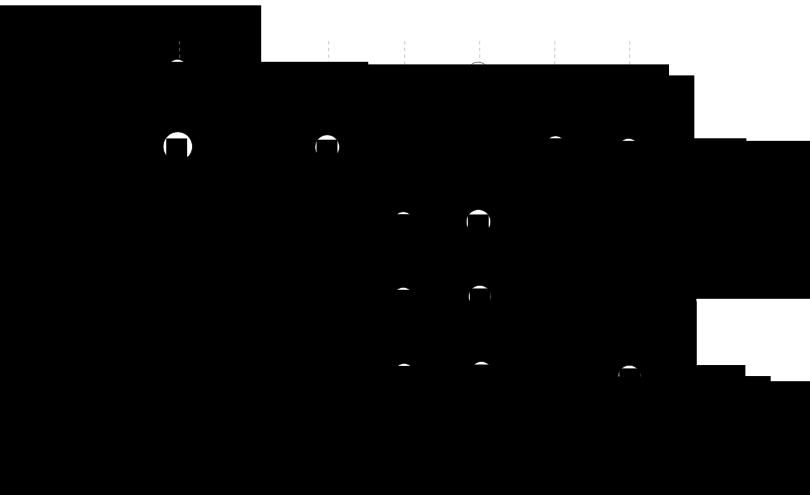
\includegraphics[width=0.99\textwidth]{figs/Facets-Contribution-MatematicalModel}
\caption{Contribution and Mathematical Model Facets}
\label{fig:Facets-Contribution-MatematicalModel}
\end{figure}   

We combined the facets {\em Contribution} and {\em Mathematical model} to determine which formal tool has been used the most to define different types of contributions (i.e., languages, models, methods), or whether there is a generic formal tool used for all types of contributions (Figure \ref{fig:Facets-Contribution-MatematicalModel}). We observed that contributions proposing algorithms  or processes for automatizing service composition use in general  heuristics or optimization category (55 papers -32.35\%). The majority of the contributions proposed composition algorithms (21 papers -12.35\%) and processes  (22 -12.9\%). The majority of contributions proposing Middleware and Process use  Petri Nets, Automata and Agents. Only 2 papers (1.18\%) propose new languages for
service-based software with NFR. 
 
 %......................................................................................
\subsubsection{Combining the facets Contribution and NFR type}
%......................................................................................

\begin{figure}[ht!]
\centering
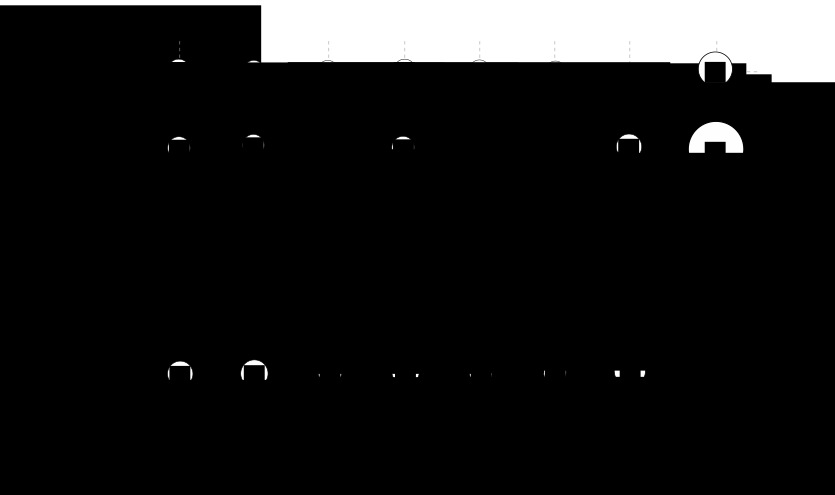
\includegraphics[width=0.99\textwidth]{figs/Facets-Contribution-NFR}
\caption{Facets Contribution and NFR Type}
\label{fig:Facets-Contribution-NFR}
\end{figure}  
       
We combined the facets {\em Contribution} and {\em NFR type} to observe the papers that (i) report solutions concerning all NFR types o just particular ones for service-based software; and (ii) the contributions that are used the most for specific NFR types (see
Figure \ref{fig:Facets-Contribution-NFR}).  First, with respect to the type of NFR, the proposals concerning general solutions that address NFR as a type of QoS are very popular (129/170papers -75.88\%). Quality properties are expressed and associated to service compositions. There are few proposals that address other NFR types  (e.g., Usability, Maintainability, Portability, Functionality, Reliability and Efficiency). Only 15 works (8.82\%) address one of
these NFR types. 

%......................................................................................
\subsubsection{Combining the facet Paradigm with the facets Contribution  and Software process development}
%......................................................................................
\begin{figure} [htpb]
\centering
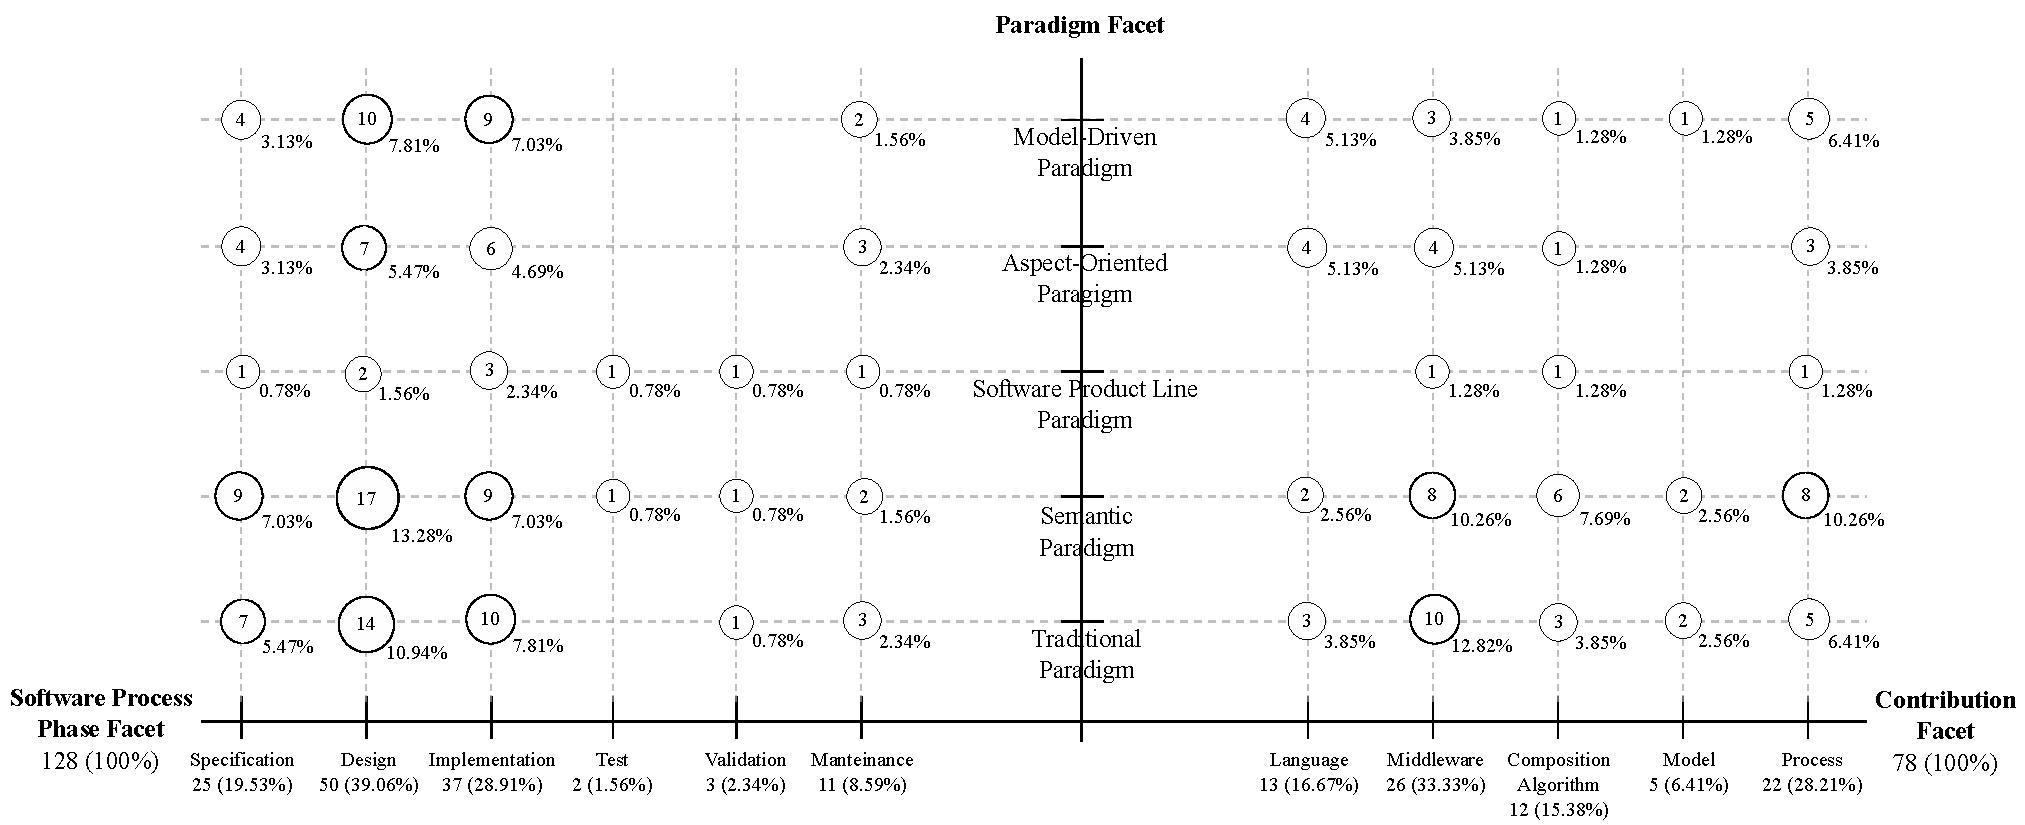
\includegraphics[width=0.99\textwidth]{figs/Facets-Paradigm-ContributionProcess}
\caption{Paradigm and Contribution/Process Facets}
\label{fig:Facets-Paradigm-ContributionProcess}
\end{figure}  

Combining the facet Paradigm with the facets Contribution and Software process development (Figure
\ref{fig:Facets-Paradigm-ContributionProcess})  it is possible to observe the phases in which software methodologies contribute to address NFR for service-based software. We also  observed whether there is a connexion between the paradigm used by methodologies with respect to the way the address NFR.
First of all, the most popular paradigms adopted by software development methodologies are Semantic with 17 papers (13:28\%), Model-Driven Development with
10 papers (7.81\%) and Traditional paradigm with 14 works (10.94\%). 
Second, the analysis shows that the phases Test and Validation are rarely addressed by methodologies independently of the adopted paradigm (2 papers for Test and 3 for Validation). In contrast, the Design, Specification and Implementation phases are addressed by a lot of methodologies independently of the adapted paradigm.
 
 %The relationship between Paradigm and the Contribution was made in the
%description of Figure \ref{fig:Facets-Contribution-ProcessParadigm}.

%......................................................................................
%\subsubsection{Combining the facets Paradigm and Mathematical Model}
%......................................................................................

%\begin{figure} [htpb]
%\centering
%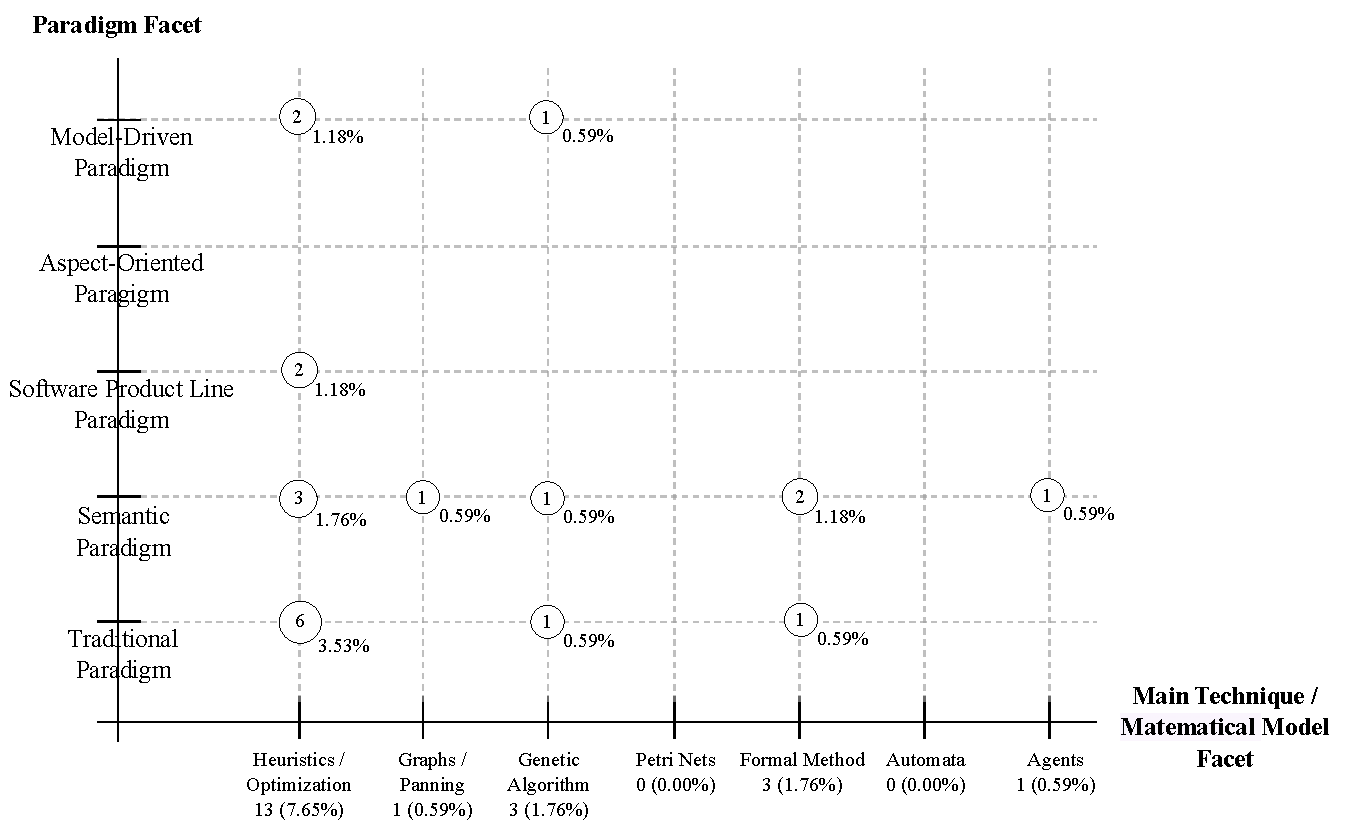
\includegraphics[width=0.9\textwidth]{figs/Facets-Paradigm-MatematicalModel}
%\caption{Paradigm and Matematical Model Facets}
%\label{fig:Facets-Paradigm-MatematicalModel}
%\end{figure}   


%Considering Figures \ref{fig:Facets-Paradigm-MatematicalModel} and
%\ref{fig:Facets-Paradigm-NFR} we can see some gaps in the relation of the
%Paradigm used and the Main Technique/Matematical Model or the NFR type
%presented. This result occurs because 76 paper, among them 170 (44.70\%)
%selected after the systematic mapping filters, could be classified in one the
%five categories of the Paradigm facet. Thus, from this point of view, there are
%some empty intersection points. For example, in Figure
%\ref{fig:Facets-Paradigm-MatematicalModel} and considering the Aspect-Oriented
%line, there is no paper which uses a mathematical model to solve problems related
%with service-based approaches in the presence of non-functional requirements.
%From Software Product Line, only two papers addresses Heuristic /
%Optimization. By one other hand, Semantic is the most used Paradigm in this
%context, representing only 4.71\% of the papers. By the other hand, the
%works which considers Semantic does not have relation with those that uses
%Petri Nets and Automata.

%......................................................................................
%\subsubsection{Combining the facets Paradigm with NFR}
%......................................................................................
%\begin{figure} [htpb]
%\centering
%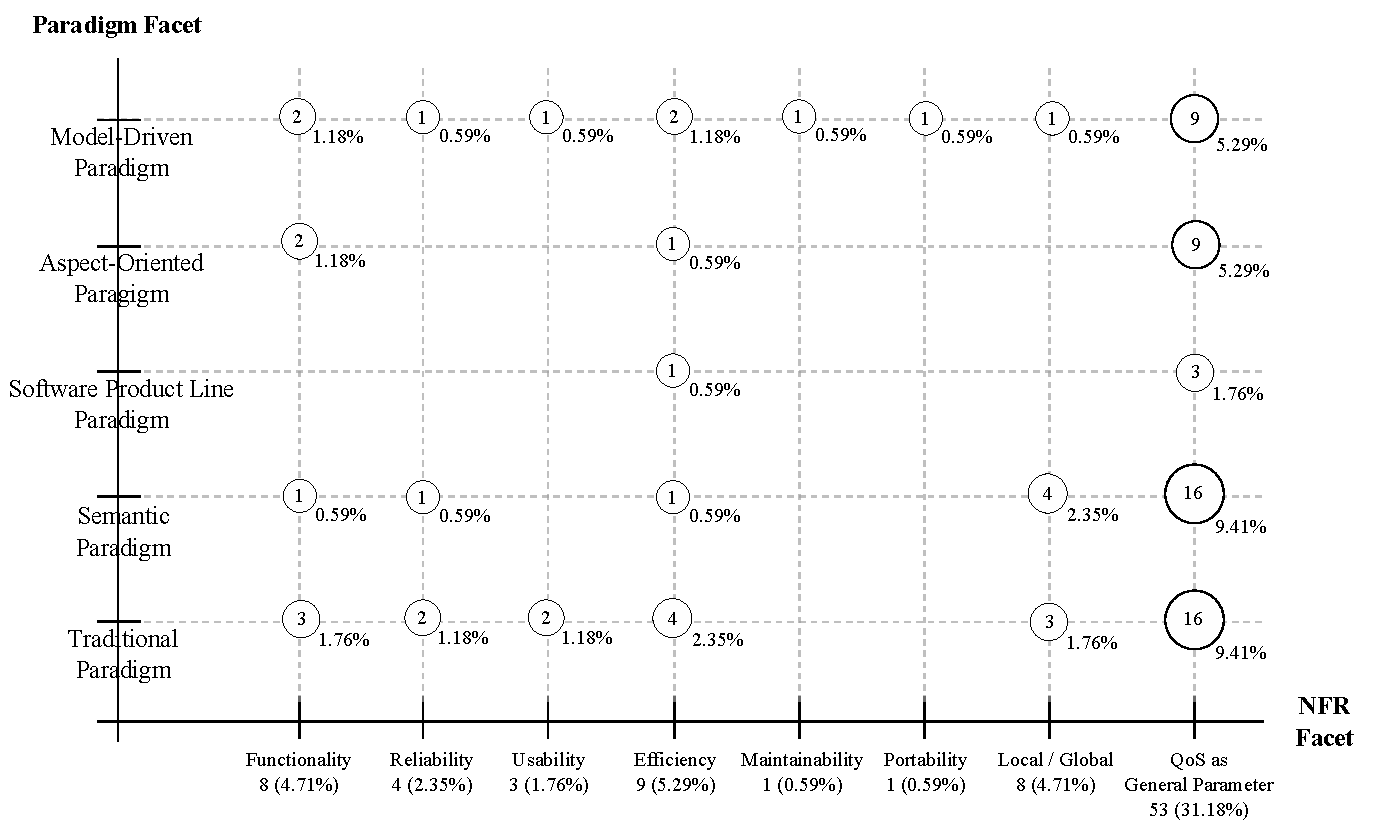
\includegraphics[width=0.9\textwidth]{figs/Facets-Paradigm-NFR}
%\caption{Paradigm and NFR Type Facets}
%\label{fig:Facets-Paradigm-NFR}
%\end{figure}   

%In Figure \ref{fig:Facets-Paradigm-NFR} we can see as similar as Figure
%\ref{fig:Facets-Contribution-NFR}, Usability, Maintainability
%and Portability are the NFR categories with less number of proposals from the
%perspective of the Paradigm facet and also the service-based composition domain.
%Eficiency and QoS are the two categories related with all Paradigm categories.
%Although, the most paper (53, representing 31.18\%) are classified using QoS.
%From these, Semantic and Traditional paradigms are the most frequent used. 
 


 
%
\bigskip

In the following sections we provide answers to the reaserch questions presented in section~\ref{sec:ResearchQuestions}.

%...............................................................................................................................................................
\subsection{RQ1: Which stages of  the service-based software development process have addressed NFR?}
%...............................................................................................................................................................

Analyzing the data presented in Figures~\ref{fig:Facets-Contribution-ProcessParadigm} and~\ref{fig:Facets-Paradigm-ContributionProcess}, we observe that NFR are considered at all stages of the software process for web applications.
However, most of the research efforts have focus on the design phase.
It is worth to notice that popular contributions are related to the organization of the software process, as well as middleware solutions.

Post-implementation phases (tests, validation and maintenance) are still to be better explored. 
Contrarily to our expectations, the testing activity is addressed by a very small number of papers.
This may indicate that either \textit{(i)} testing NFR compliance do not require specific techniques or \textit{(ii)} there is a research opportunity/challenge in this area.

Semantic tools (such as ontologies) are the preferred method for supporting NFR in web applications.
Although the usage of model-driven techniques is significant, we have not identified papers reporting on testing and validation using this approach. 
We believe that this is an area that deserves further investigation.

Our study shows a lack of testing NFRs using traditional software engineering methods for web applications.
This is not surprising since traditional testing techniques deal with functional requirements.

Another conspicuous absence is related to the support given by service composition languages to the testing and validation phases of software development. 
Some recent initiatives (such as~\cite{piSOD-M}) deals with this problem.



%...............................................................................................................................................................
\subsection{RQ2: What type of solutions have been proposed over the years to deal with NFR for service-based software?}
%...............................................................................................................................................................
Represent, specify and implement ...

%...............................................................................................................................................................
\subsection{RQ3 : Which is the scope of existing solutions for addressing NFR?}
%...............................................................................................................................................................
 Global/local and NFR types (one or several NFRs).
 
%\subsection{Research gaps and open issues}




%..--..--..--..--..--..--..--..--..--..--..--..--..--..--..--..--..--..--..--..--..--..--..--..--..--..--..--..--..--..--..--..--..--..--..--..--..--..--


%*********************************************************************************************************
\section{Concluding remarks}\label{sec:conclusions}
The mapping results presented can be the starting point
to motivate new studies, support the investigation of specific problems not sufficiently explored yet. The quantitative analysis provides an idea of the trends in service-based software development with NFR, including methodologies, languages and tools. The distribution of the papers that deal with NFR shows that they are addressed in different domains but  the vocabulary changes a lot and that there is a need of consensus, despite the existence of specifications like ISO/IEC 9126. When NFR are addressed at the level of the services they are related to QoS measures like economy or economic cost, availability, authentication requirements for contacting a service. NFR as defined by ISO/IEC 9126 are vast and papers address one or two at a time, particularly those related to the software engineering domain. Middleware solutions provide frameworks that consider different types of NFR but this concerns only the implementation stage of the software development process. This implies that the compliance between the design and the implementation might not be ensured.

With respect to the systematic mapping, we think that it requires a qualitative perspective that can be added by explicitly adding filtering and clustering criteria related to the provenance of the papers, the impact factor of the conference/journal where they appear, the reputation of the authors (given for example by their H factor), the institution and country of the authors. Without discarding the quantitative analysis, adding these criteria could increase the quality and value of the analysis. Similarly, we feel that choosing key words in the second phase of the methodology can be empirical, using vocabularies of the knowledge domain, could help to have a more representative choice. We are currently working in providing tools that can help to add quality to the systematic mapping method.



%% References with bibTeX database:

\bibliographystyle{plain}
\bibliography{bibliography,papersSistMapping}


\end{document}

%%
%% End of file `elsarticle-template-1a-num.tex'.
